\documentclass[border=2mm,12pt,tikz]{standalone}
\usepackage{tikz-3dplot}
\usetikzlibrary{fpu}
\def\pgfmathsetmacroFPU#1#2{\begingroup%
\pgfkeys{/pgf/fpu,/pgf/fpu/output format=fixed}%
\pgfmathsetmacro{#1}{#2}%
\pgfmathsmuggle#1\endgroup}%
\begin{document}
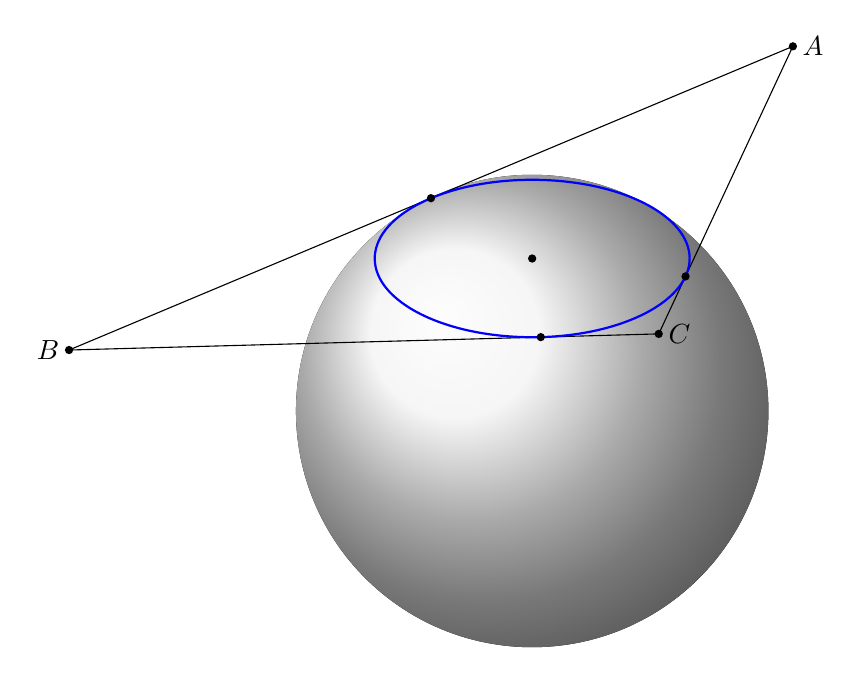
\begin{tikzpicture}[scale=1/2,declare
    function={a=15;b=15;c=24;R=6;}]
 \path (0,0,0)  coordinate  (O);
 % compute radius of incircle
 \pgfmathsetmacroFPU{\saux}{(a+b+c)/2}
 \pgfmathsetmacroFPU{\inradius}{sqrt(\saux*(\saux-a)*(\saux-b)*(\saux-c))/\saux}
 % compute height of circle
 \pgfmathsetmacro{\haux}{sqrt(R*R-\inradius*\inradius)}
 % compute angles of triangle
 \pgfmathsetmacro{\alphaaux}{acos((b*b+c*c-a*a)/(2*b*c))}
 \pgfmathsetmacro{\betaaux}{acos((a*a+c*c-b*b)/(2*a*c))}
 \pgfmathsetmacro{\gammaaux}{acos((a*a+b*b-c*c)/(2*a*b))}
 % compute distances from the corners of the triangle to the points where
 % the triangle touches the circle
 \pgfmathsetmacro{\touchA}{(b+c-a)/2}
 \pgfmathsetmacro{\touchB}{(a+c-b)/2}
 \pgfmathsetmacro{\touchC}{(a+b-c)/2}
 \tdplotsetmaincoords{60}{140}
 \begin{scope}[tdplot_main_coords]
  \fill[ball color=gray!10,tdplot_screen_coords] (O)  circle[radius=6];
  \path (-\touchA,-\inradius,\haux) coordinate[label=right:$A$](A)
   (\touchB,-\inradius,\haux) coordinate[label=left:$B$](B)
   ({-\touchA+cos(\alphaaux)*b},{-\inradius+sin(\alphaaux)*b},\haux)
     coordinate[label=right:$C$](C)
   (0,-\inradius,\haux) coordinate (TAB)
   ({-\touchA+cos(\alphaaux)*\touchA},{-\inradius+sin(\alphaaux)*\touchA},\haux)
    coordinate (TAC)
   ({\touchB+cos(180-\betaaux)*\touchB},{-\inradius+sin(180-\betaaux)*\touchB},\haux)
    coordinate (TBC)
    (0,0,\haux) coordinate (M);
  \draw (A) -- (B) -- (C) -- cycle;
  \begin{scope}[canvas is xy plane at z=\haux]
   \draw[blue,thick] (M) circle[radius=\inradius];
  \end{scope}
  \foreach \X in {A,B,C,M,TAB,TAC,TBC}
  {\fill (\X) circle[radius=3pt];}
 \end{scope}
\end{tikzpicture}
\end{document}
